% Ch9 rates / max-min diagrams, redrawn in TikZ from the original papers
\usetikzlibrary{calc,arrows.meta,angles,quotes}
\tikzset{c9/.style={line width=0.7pt},c9d/.style={dashed,line width=0.5pt},c9a/.style={-{Stealth[length=2mm]},line width=0.5pt},c9aa/.style={{Stealth[length=2mm]}-{Stealth[length=2mm]},line width=0.5pt}}
\newcommand{\rtmark}[3]{\draw[line width=0.4pt] ($(#1)!#3!(#2)$) -- ($($(#1)!#3!(#2)$)!#3!90:(#2)$) -- ($(#1)!#3!90:(#2)$);}
% TJC 2025 P2 Q4: Figures 1 and 2
\newcommand{\figTJCfa}{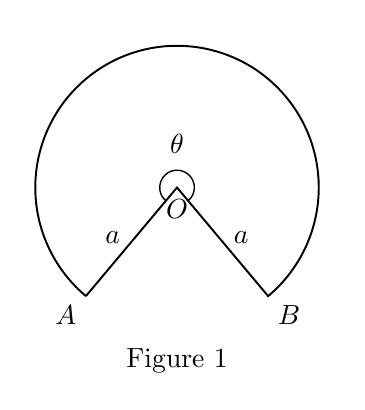
\begin{tikzpicture}[scale=1]
\coordinate (O) at (0,0); \coordinate (A) at (230:1.8); \coordinate (B) at (310:1.8);
\draw[c9] (A) -- (O) -- (B) arc[start angle=310,end angle=590,radius=1.8];
\draw[line width=0.5pt] (310:0.22) arc[start angle=310,end angle=590,radius=0.22];
\node at (0,0.55) {$\theta$}; \node[below=1pt] at (O) {$O$};
\node at ($(O)!0.55!(A)+(-0.18,0.12)$) {$a$}; \node at ($(O)!0.55!(B)+(0.18,0.12)$) {$a$};
\node[below left] at (A) {$A$}; \node[below right] at (B) {$B$};
\node at (0,-2.2) {Figure 1};
\end{tikzpicture}}
\newcommand{\figTJCfb}{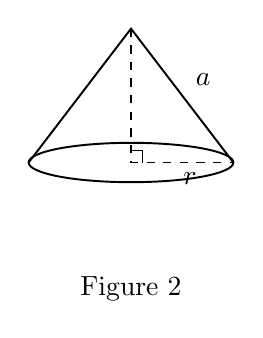
\begin{tikzpicture}[scale=1]
\draw[c9] (0,0) ellipse (1.3 and 0.25); \draw[c9] (-1.3,0) -- (0,1.7) -- (1.3,0);
\draw[c9d] (0,1.7) -- (0,0) -- (1.3,0); \draw[line width=0.4pt] (0,0.15)--(0.15,0.15)--(0.15,0);
\node[above right] at (0.7,0.85) {$a$}; \node[below] at (0.75,0) {$r$};
\node at (0,-1.6) {Figure 2};
\end{tikzpicture}}
% TJC 2025 P2 Q4: Figure 3 (two cones tip-to-tip)
\newcommand{\figTJCfc}{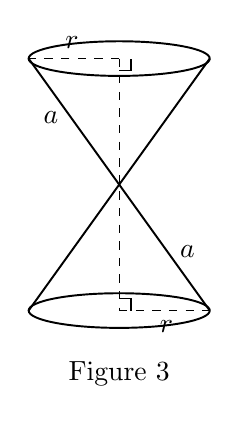
\begin{tikzpicture}[scale=1]
\draw[c9] (0,1.6) ellipse (1.15 and 0.22); \draw[c9] (0,-1.6) ellipse (1.15 and 0.22);
\draw[c9] (-1.15,1.6) -- (1.15,-1.6); \draw[c9] (1.15,1.6) -- (-1.15,-1.6);
\draw[c9d] (0,1.6) -- (0,-1.6); \draw[c9d] (0,1.6) -- (-1.15,1.6); \draw[c9d] (0,-1.6) -- (1.15,-1.6);
\draw[line width=0.4pt] (0,1.45)--(0.15,1.45)--(0.15,1.6); \draw[line width=0.4pt] (0,-1.45)--(0.15,-1.45)--(0.15,-1.6);
\node[above] at (-0.6,1.6) {$r$}; \node[below] at (0.6,-1.6) {$r$};
\node[left] at (-0.65,0.85) {$a$}; \node[right] at (0.65,-0.85) {$a$};
\node at (0,-2.4) {Figure 3};
\end{tikzpicture}}
% DHS 2025 P1 Q11: tank
\newcommand{\figDHSa}{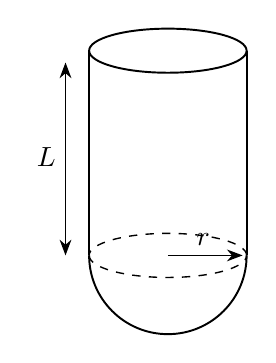
\begin{tikzpicture}[scale=1]
\draw[c9] (0,2.6) ellipse (1 and 0.28);
\draw[c9] (-1,2.6) -- (-1,0); \draw[c9] (1,2.6) -- (1,0);
\draw[c9d] (1,0) arc[start angle=0,end angle=180,x radius=1,y radius=0.28];
\draw[c9d] (-1,0) arc[start angle=180,end angle=360,x radius=1,y radius=0.28];
\draw[c9] (-1,0) arc[start angle=180,end angle=360,radius=1];
\draw[c9aa] (-1.3,2.45) -- (-1.3,0); \node[left] at (-1.3,1.25) {$L$};
\draw[c9a] (0,0) -- (0.95,0); \node[above] at (0.45,0) {$r$};
\end{tikzpicture}}
% DHS 2025 P1 Q11: hemispherical bottom with water
\newcommand{\figDHSb}{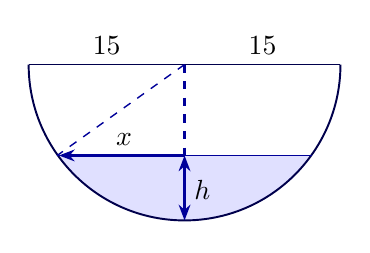
\begin{tikzpicture}[scale=1.1,blue!60!black]
\fill[blue!12] (-1.47,-1.05) arc[start angle=215.7,end angle=324.3,radius=1.8] -- cycle;
\draw[c9,black!70!blue] (-1.8,0) -- (1.8,0); \draw[c9,black!70!blue] (-1.8,0) arc[start angle=180,end angle=360,radius=1.8];
\node[black,above] at (-0.9,0) {15}; \node[black,above] at (0.9,0) {15};
\draw[c9d,thick] (0,0) -- (0,-1.05); \draw[c9d] (0,0) -- (-1.47,-1.05);
\draw[line width=0.6pt] (-1.47,-1.05) -- (1.47,-1.05);
\draw[c9a,thick] (0,-1.05) -- (-1.45,-1.05); \node[black,above] at (-0.7,-1.05) {$x$};
\draw[c9aa,thick] (0,-1.05) -- (0,-1.8); \node[black,right] at (0,-1.45) {$h$};
\end{tikzpicture}}
% DHS solution (c)(i) diagram
\newcommand{\figDHSsol}{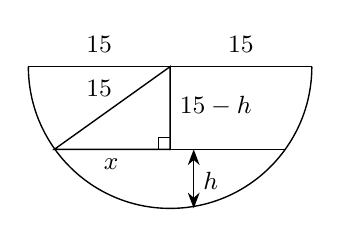
\begin{tikzpicture}[scale=1]
\draw[line width=0.5pt] (-1.8,0) -- (1.8,0); \draw[line width=0.5pt] (-1.8,0) arc[start angle=180,end angle=360,radius=1.8];
\node[above] at (-0.9,0.05) {\small 15}; \node[above] at (0.9,0.05) {\small 15};
\draw[line width=0.5pt] (0,0) -- (-1.47,-1.05) -- (0,-1.05) -- cycle; \draw[line width=0.4pt] (0,-0.9)--(-0.15,-0.9)--(-0.15,-1.05);
\draw[line width=0.5pt] (-1.47,-1.05) -- (1.47,-1.05);
\node[above] at (-0.9,-0.5) {\small 15}; \node[right] at (0,-0.5) {\small $15-h$}; \node[below] at (-0.75,-1.05) {\small $x$};
\draw[c9aa] (0.3,-1.05) -- (0.3,-1.8); \node[right] at (0.3,-1.45) {\small $h$};
\end{tikzpicture}}
% TJC 2024 Promo Q12: sphere inscribed in inverted cone
\newcommand{\figTJCsph}[1][0]{\begin{tikzpicture}[scale=1]
\coordinate (A) at (0,-3); \coordinate (C) at (-1.6,0); \coordinate (B) at (1.6,0); \coordinate (O) at (0,0); \coordinate (P) at (0,-0.96);
\coordinate (D) at ($(C)!(P)!(A)$);
\draw[c9] (O) ellipse (1.6 and 0.45); \draw[c9] (C) -- (A) -- (B); \draw[c9] (P) circle (0.96);
\draw[c9d] (C) -- (O); \draw[c9d] (O) -- (A); \draw[c9d] (P) -- (D);
\rtmark{O}{C}{0.13} \rtmark{D}{P}{0.11}
\node[above,font=\small,inner sep=1pt] at (-0.8,0.02) {$r$ cm}; \node[above right,inner sep=1pt] at (0.05,0.02) {$O$};
\node[above,font=\small,inner sep=1pt] at ($(P)!0.55!(D)+(0.05,0.05)$) {$R$ cm};
\ifnum#1=0 \draw[c9aa,dotted] (2.1,0.1) -- (2.1,-3); \node[right] at (2.1,-1.45) {$h$ cm};
\else \node[left] at (C) {$C$}; \node[right] at (B) {$B$}; \node[below left] at (D) {$D$}; \node[below] at (A) {$A$}; \node[right] at (P) {$P$}; \node[right] at (0.1,-0.6) {$h$ cm};\fi
\end{tikzpicture}}
% CJC 2024 Promo Q10: paper cone cup
\newcommand{\figCJC}{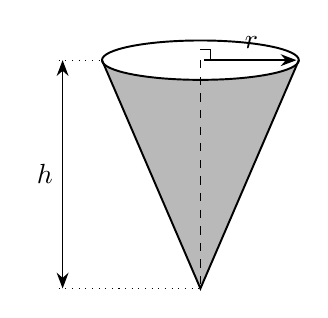
\begin{tikzpicture}[scale=1]
\fill[gray!55] (-1.25,0) -- (0,-2.9) -- (1.25,0) arc[start angle=0,end angle=-180,x radius=1.25,y radius=0.25];
\draw[c9,fill=white] (0,0) ellipse (1.25 and 0.25); \draw[c9] (-1.25,0) -- (0,-2.9) -- (1.25,0);
\draw[c9d] (0,0) -- (0,-2.9); \draw[line width=0.4pt] (0,0.13)--(0.13,0.13)--(0.13,0);
\draw[c9a] (0.05,0) -- (1.22,0); \node[above] at (0.65,0.02) {$r$};
\draw[line width=0.4pt,dotted] (-1.8,0) -- (-1.25,0); \draw[line width=0.4pt,dotted] (-1.8,-2.9) -- (0,-2.9);
\draw[c9aa,line width=0.6pt] (-1.75,0) -- (-1.75,-2.9); \node[left] at (-1.75,-1.45) {$h$};
\end{tikzpicture}}
% CJC solution (d) diagram
\newcommand{\figCJCsol}{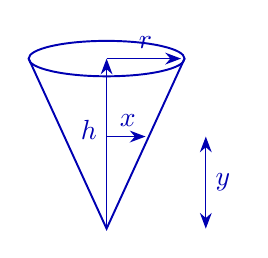
\begin{tikzpicture}[scale=0.9,blue!70!black]
\draw[line width=0.7pt] (0,0) ellipse (1.1 and 0.25); \draw[line width=0.7pt] (-1.1,0) -- (0,-2.4) -- (1.1,0);
\draw[c9a] (0,-2.4) -- (0,0); \draw[c9a] (0,0) -- (1.05,0); \node[above] at (0.55,0) {$r$}; \node[left] at (0,-1) {$h$};
\draw[c9a] (0,-1.1) -- (0.55,-1.1); \node[above] at (0.3,-1.1) {$x$};
\draw[c9aa] (1.4,-1.1) -- (1.4,-2.4); \node[right] at (1.4,-1.75) {$y$};
\end{tikzpicture}}
% EJC 2018 Promo Q7: right cone, slant edge R
\newcommand{\figEJC}{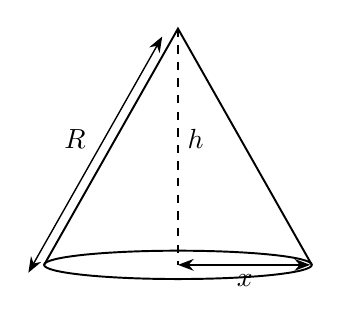
\begin{tikzpicture}[scale=1]
\draw[c9] (0,0) ellipse (1.7 and 0.18); \draw[c9] (-1.7,0) -- (0,3) -- (1.7,0);
\draw[c9d] (0,3) -- (0,0); \draw[c9aa] (0,0) -- (1.68,0); \node[below] at (0.85,0) {$x$};
\draw[c9aa] ($(-1.7,0)+(-0.2,-0.1)$) -- ($(0,3)+(-0.2,-0.1)$); \node[left] at (-1.05,1.6) {$R$}; \node[right] at (0,1.6) {$h$};
\end{tikzpicture}}
% TMJC 2024 Prelim P1 Q2: cylinder inscribed in sphere
\newcommand{\figTMJC}{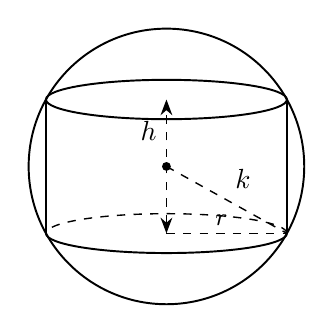
\begin{tikzpicture}[scale=1]
\draw[c9] (0,0) circle (1.75);
\draw[c9] (0,0.85) ellipse (1.53 and 0.25); \draw[c9] (-1.53,0.85) -- (-1.53,-0.85); \draw[c9] (1.53,0.85) -- (1.53,-0.85);
\draw[c9] (-1.53,-0.85) arc[start angle=180,end angle=360,x radius=1.53,y radius=0.25];
\draw[c9d] (1.53,-0.85) arc[start angle=0,end angle=180,x radius=1.53,y radius=0.25];
\draw[c9aa,dashed] (0,-0.85) -- (0,0.85); \node[left] at (0,0.45) {$h$};
\fill (0,0) circle (1.6pt); \draw[c9d] (0,0) -- (1.53,-0.85); \node[above right] at (0.75,-0.4) {$k$};
\draw[c9d] (0,-0.85) -- (1.53,-0.85); \node[above] at (0.7,-0.88) {\small$r$};
\end{tikzpicture}}
% TMJC solution triangle
\newcommand{\figTMJCsol}{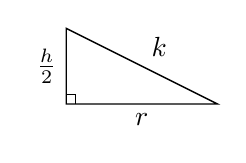
\begin{tikzpicture}[scale=0.8]
\draw[line width=0.5pt] (0,0) -- (2.4,0) -- (0,1.2) -- cycle; \draw[line width=0.4pt] (0,0.15)--(0.15,0.15)--(0.15,0);
\node[left] at (0,0.6) {$\frac{h}{2}$}; \node[below] at (1.2,0) {$r$}; \node[above right] at (1.2,0.6) {$k$};
\end{tikzpicture}}
% RVHS 2025 Promo Q1 solution diagram (conical tank with water)
\newcommand{\figRVHSsol}{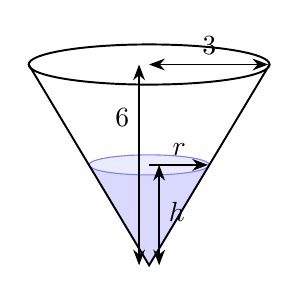
\begin{tikzpicture}[scale=0.85]
\fill[blue!15] (-0.9,-1.5) -- (0,-3) -- (0.9,-1.5) arc[start angle=0,end angle=-180,x radius=0.9,y radius=0.15];
\draw[blue!50,fill=blue!8] (0,-1.5) ellipse (0.9 and 0.15);
\draw[c9] (0,0) ellipse (1.8 and 0.3); \draw[c9] (-1.8,0) -- (0,-3) -- (1.8,0);
\draw[c9aa] (0,0) -- (1.78,0); \node[above] at (0.9,0) {$3$};
\draw[c9aa] (-0.15,0) -- (-0.15,-3); \node[left] at (-0.15,-0.8) {$6$};
\draw[c9a] (0,-1.5) -- (0.88,-1.5); \node[above] at (0.45,-1.5) {$r$};
\draw[c9aa] (0.15,-1.5) -- (0.15,-3); \node[right] at (0.15,-2.2) {$h$};
\end{tikzpicture}}
